
%(BEGIN_QUESTION)
% Copyright 2009, Tony R. Kuphaldt, released under the Creative Commons Attribution License (v 1.0)
% This means you may do almost anything with this work of mine, so long as you give me proper credit

Analyze this data frame for a 7-bit NRZ data frame with odd parity and answer the questions that follow:

$$
\includegraphics[width=15.5cm]{i03798x01.eps}$$

\begin{itemize}
\item{} Express the 7-bit data in hexadecimal form: \underbar{\hskip 50pt}
\vskip 5pt
\item{} Does the parity bit suggest the data integrity is good? ({\it Yes / No})
\vskip 5pt
\item{} Identify the location of the {\it start} bit
\vskip 5pt
\item{} Identify the location of the {\it stop} bit
\vskip 5pt
\item{} Identify the minimum received voltage levels corresponding to {\it mark} and {\it space} if this is an RS-232 network
\end{itemize}

\underbar{file i03798}
%(END_QUESTION)





%(BEGIN_ANSWER)

$$\includegraphics[width=15.5cm]{i03798x02.eps}$$

\begin{itemize}
\item{} Express the 7-bit data in hexadecimal form: {\tt 7B}
\vskip 5pt
\item{} Does the parity bit suggest the data integrity is good? ({\bf No})
\vskip 5pt
\item{} Identify the minimum received voltage levels corresponding to {\it mark} and {\it space} if this is an RS-232 network ({\bf Mark = -3 V ; Space = +3 V})
\end{itemize}

I suggest 3 points for the proper hexadecimal translation, 3 points for parity check, and 1 point each for correctly identifying the start and stop bits, and 2 points for correct mark and space voltages.

%(END_ANSWER)





%(BEGIN_NOTES)

{\bf This question is intended for exams only and not worksheets!}.

%(END_NOTES)


